\subsection{Introducción:}

\begin{itemize}
\item [\textit{a)}] Completar \textit{inicializar\_mmu} que se encargue de inicializar las estructuras globales necesarias para administrar la memoria en el área libre (un contador de páginas libres).
\item [\textit{b)}] Completar la función \textit{mmu\_inicializar\_memoria\_perro}.
\end{itemize}

\subsection{Ítem a): Completar \textit{inicializar\_mmu}.}

	Para realizar esta función simplemente creamos en el archivo \textit{mmu.c} las variables globales las cuales puden ser usadas por el resto de las funciones:	

	$~$

	uint pagLibre = 0x100000 

	uint cantPagLibre = 768 

	uint paginaJugadorA

	uint paginaJugadorB\\

\subsection{Ítem b): Completar la función \textit{mmu\_inicializar\_memoria\_perro}.}

La función la realizamos de la siguiente manera:

\begin{figure}[H]
\begin{center}
\minipage{1.05\textwidth}
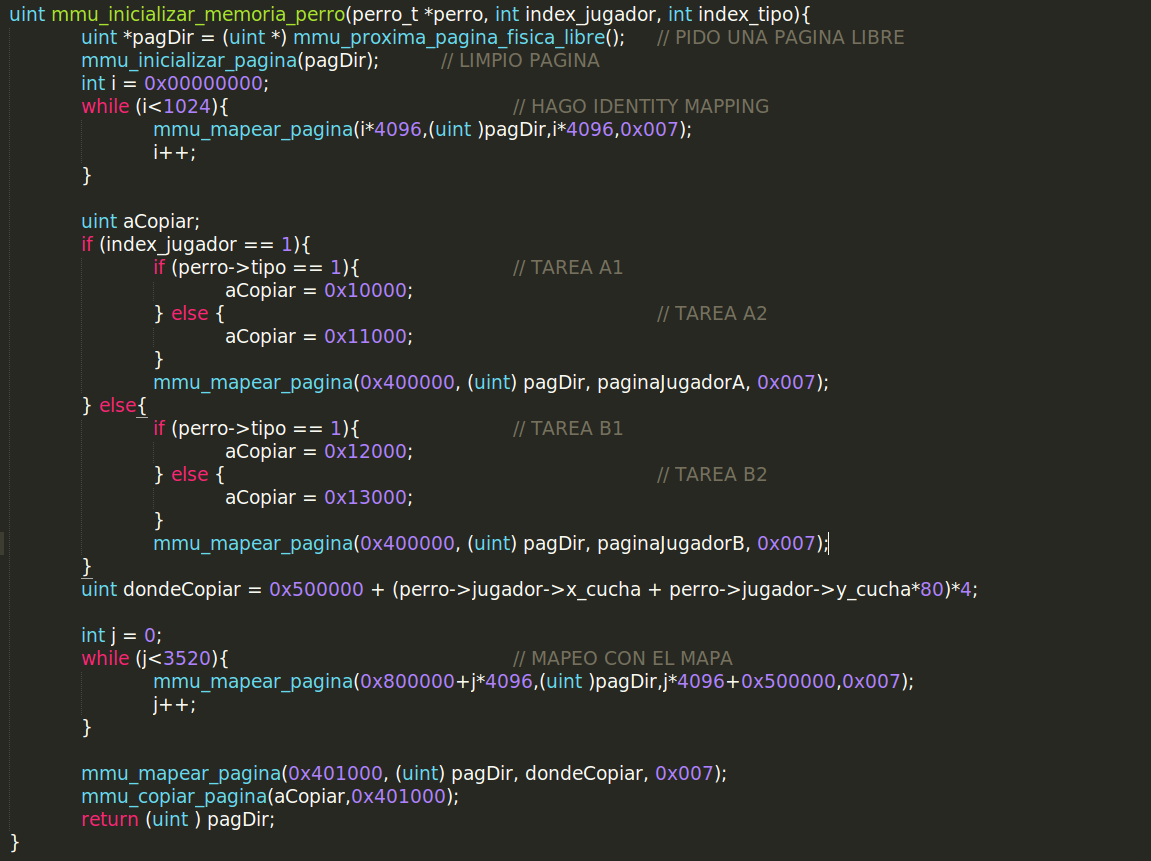
\includegraphics[width=\linewidth]{ejercicio4/funprin.png}
\caption{{\small Función principal} }
\endminipage
\end{center}
\end{figure}


La función realiza lo siguiente: 

\begin{itemize}

	\item[A:] Recibe como parametros un perro, un int que sirve para indicar que jugador es y otro int para identificar el tipo de perro.

	\item[B:] Comienza pidiendo un lugar para crear una página libre, para eso llama a la función \textit{mmu\_proxima\_pagina\_fisica\_libre()}. Una vez obtenida la posicion, procede a crear la pagina y luego la mapea con la funcion \textit{mmu\_mapear\_pagina}

	\begin{figure}[H]
	\begin{center}
	\minipage{0.65\textwidth}
	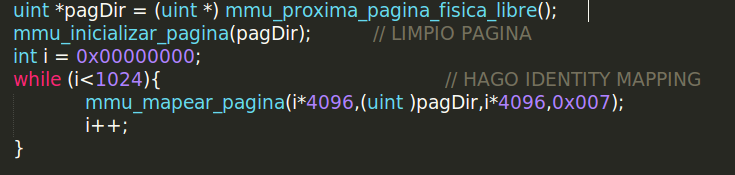
\includegraphics[width=\linewidth]{ejercicio4/fun1}
	\caption{{\small } }
	\endminipage
	\end{center}
	\end{figure}

	\item[C:]  Luego, para saber que tarea copiar identifica que jugador es, usando el parámetro de entrada \textit{index\_jugador}, luego identifica que tipo de perro es , usando la variable de entrada \textit{index\_tipo}. Con esa informacion, la función sabe donde esta la tarea que tiene que copiar. Ademá es necesario que se le mapee esta nueva tarea al jugador correspondiente por eso, dependiendo de que jugador sea, se le mapea esta nueva tarea.
	 
	\begin{figure}[H]
	\begin{center}
	\minipage{0.7\textwidth}
	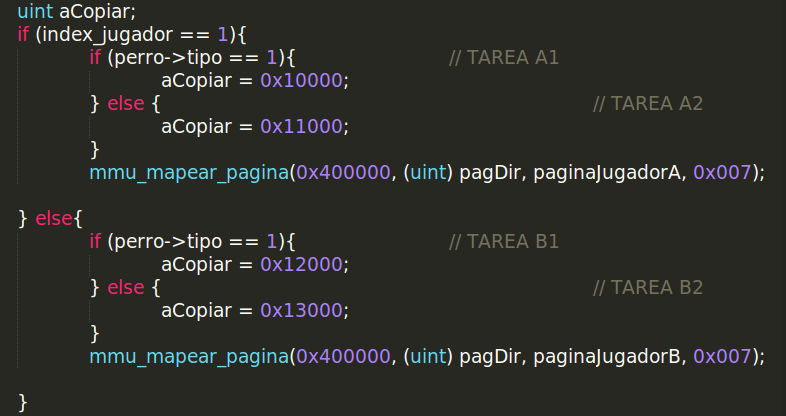
\includegraphics[width=\linewidth]{ejercicio4/fun2}
	\caption{{\small } }
	\endminipage
	\end{center}
	\end{figure}

	\item[D:] Después de mapear el mapa devuelta es necesario mapear la dirección 0X401000 con la posición donde tiene que estar la tarea. Para saber en que dirección tiene que estar la tarea (o sea dónde va a estar el perro), la función toma la posición 0x500000 (posición donde se encuentra el mapa) y le suma el valor X y el valor Y de la cucha del perro y mapea 0X401000 con la dirección obtenida. De esta manera el kernel sabe donde deben estar los perros y finalmente se puede copiar la tarea a la dirección 0X401000, la cual va a estar mapeada correctamente al lugar donde hay que poner a los nuevos perros/tareas.
	
\end{itemize}